%%%%%%%%%%%%%%%%%%%%%%%%%%%%%%%%%%%%%%%%%%%%%%%%%%%%%%%%%%%%%%%%%%%%%%%%%%%%%%%%%%%%%%%%%%%%%%%%%%%%%%%%%%%%%%%%
%% AAMAS 2027 submission draft (anonymous).
%% Compile on Overleaf with the official AAMAS 2027 template: put aamas.cls (and the other files of
%% aamas_2027_template.zip) next to this file. If the template's own sample file has a different front matter
%% (the \acm... lines below), copy ITS front matter over this block; the body does not depend on it.
%% Values still to come from the full run (notebooks part A and B) are typeset in red with \tbd{...}.
%%%%%%%%%%%%%%%%%%%%%%%%%%%%%%%%%%%%%%%%%%%%%%%%%%%%%%%%%%%%%%%%%%%%%%%%%%%%%%%%%%%%%%%%%%%%%%%%%%%%%%%%%%%%%%%%
\documentclass[sigconf]{aamas}

\usepackage{balance}
\usepackage{booktabs}
\usepackage{multirow}
\usepackage{amsmath}

\newcommand{\tbd}[1]{\textcolor{red}{#1}}
\newcommand{\sys}{\textsc{PreGate}}

%%% ---------------- front matter (replace with the official template's if it differs) ----------------
\setcopyright{ifaamas}
\acmConference[AAMAS '27]{Proc.\@ of the 26th International Conference
on Autonomous Agents and Multiagent Systems (AAMAS 2027)}{May 3 -- 7, 2027}
{Hanoi, Vietnam}{}
\copyrightyear{2027}
\acmYear{2027}
\acmDOI{}
\acmPrice{}
\acmISBN{}
\acmSubmissionID{<<submission id>>}

\title[Verify Before You Schedule]{Verify Before You Schedule: A Small-Model Verifier\\for LLM Agents Acting in Time-Evolving Smart Homes}

\author{Paper \#XXX}
\affiliation{}
%%% -------------------------------------------------------------------------------------------------------------

\begin{abstract}
LLM agents that control smart homes must turn requests such as ``dim the light 8 minutes after the previous
action'' or ``pause the dishwasher when the dryer finishes'' into correctly timed device commands. On the
SimuHome benchmark, current agents fail most often on exactly these scheduling tasks: they rarely notice when a
request's time constraints contradict each other, and the scheduling tool accepts any plan, so wrong times and
failing commands surface only when the action fires. We present \sys{}, a verification layer that wraps an
unmodified agent's tool interface. Before the agent starts, a fine-tuned small language model (1.7B parameters)
translates the request into time constraints, device finish times are read from the home, and an SMT solver
either proves the request contradictory or computes an allowed time window for every requested action.
Contradictory requests are answered without any large-model call, or the agent is warned once. While the agent
works, every scheduling call is checked against these windows and dry-run on a copy of the home, and refused
calls come back with an actionable fix: the correct time range, the device's real command signature, or the
state that makes the action a no-op. On all 300 SimuHome scheduling episodes with a Qwen2.5-14B agent and a
5-fold cross-validated parser, \sys{} handles 130 of 150 contradictory requests correctly (agent alone: 9; a
self-check prompt: 19), with almost no large-model calls on two of three sub-types, and completes 15 of 148
feasible requests against 2 for the agent alone and 1 with self-check ($p<0.001$, paired). Almost every gain on
feasible requests follows a refusal that showed the agent the device's real command signature.
\end{abstract}

\keywords{LLM agents; runtime verification; neuro-symbolic AI; small--large model collaboration; SMT;
smart homes; IoT}

\begin{document}
\pagestyle{fancy}
\fancyhead{}
\maketitle

%%%%%%%%%%%%%%%%%%%%%%%%%%%%%%%%%%%%%%%%%%%%%%%%%%%%%%%%%%%%%%%%%%%%%%%%%%%%%%%%%%%%%%%%%%%%%%%%%%%%%%%%%%%%%%%%
\section{Introduction}

Large language models (LLMs) are increasingly deployed as agents that act on physical environments through tool
APIs, and the smart home is one of the most direct examples: the agent reads device states, issues commands and
schedules actions on behalf of a user. Many everyday requests are \emph{temporal}. They chain actions
(``turn on the fan in 20 minutes and raise it to 50\% 23 minutes after that''), refer to device events
(``start the washer 10 minutes after the dishwasher finishes'') or coordinate devices (``start the dryer now and
pause it when the other dryer finishes''). Serving such a request requires reasoning about clock times,
offsets and device run times, and then emitting device commands with exactly the right arguments.

SimuHome~\cite{seo2026simuhome} measures this ability in a simulated, time-evolving home built on the Matter
device standard. Its authors find workflow scheduling to be the most persistent challenge across all task types
and identify two structural problems. First, agents suffer from \emph{contradiction blindness}: when a request's
time constraints cannot all be satisfied (e.g., ``at 12:23, which is 12 minutes from now'' when it is 12:15),
the agent schedules one reading and reports success instead of pointing out the conflict. Second, the scheduling
tool only confirms that a workflow was registered; whether its steps will execute is discovered only when it
fires, so ``agents cannot detect erroneous plans''. Self-correction prompts and fine-tuning bring limited gains,
and the authors suggest, as future work, testing plans in the simulator before committing them.

We argue that both problems are better addressed \emph{outside} the large model, at the boundary between the
agent and its tools, by components that can check rather than guess. Temporal consistency of a request is a
satisfiability question over a handful of linear constraints, which an SMT solver decides exactly once the
request is formalized. Whether a scheduled workflow will execute, and what state it will produce, can be
determined by running it on a copy of the home. Neither check needs a large model, and both can return precise,
actionable feedback.

This paper presents \sys{}, a verification layer for LLM agents that act through scheduling tools. \sys{} pairs
a large agent model with a small language model and a solver (Figure~\ref{fig:arch}). The small model translates
the request into a structured intermediate representation (IR) of goals and time readings; deterministic rules
ground the IR in the request text and the home's device list; Z3~\cite{demoura2008z3} decides satisfiability and
computes an allowed time window per goal. A gate around the agent's scheduling tool then verifies every call
the agent makes. Our contributions are:
\begin{itemize}
  \item A \textbf{two-phase verification method} that wraps an unmodified, black-box agent: a request-level
  satisfiability proof before the agent acts, and plan-level checks whose specifications are derived
  automatically from each request rather than written by hand.
  \item A \textbf{small--large model collaboration} in which a 1.7B-parameter model and a solver decide
  contradictory requests with zero large-model calls, and supervise the large model's actions otherwise.
  \item \textbf{Actionable refusals} grounded in simulation: allowed time ranges (including deadline semantics),
  the device's real command signatures, and no-effect detection by comparing the home with and without the call.
  \item An \textbf{evaluation protocol} for agents on real-time simulators that removes hosted-API latency as a
  confound, with a 5-fold cross-validated parser and paired comparisons on all 300 SimuHome scheduling episodes,
  together with an analysis of why agents fail on feasible scheduling requests.
\end{itemize}
On all 300 SimuHome scheduling episodes with a 14B-parameter agent, \sys{} raises correct handling of
contradictory requests from 9 to 130 of 150, with almost no large-model calls on two of the three sub-types,
while a self-check prompt reaches 19. On feasible requests it is the only configuration that helps (15 of 148
completed, against 2 for the agent alone), and the gains follow directly from refusals that told the agent the
device's real command signature.

%%%%%%%%%%%%%%%%%%%%%%%%%%%%%%%%%%%%%%%%%%%%%%%%%%%%%%%%%%%%%%%%%%%%%%%%%%%%%%%%%%%%%%%%%%%%%%%%%%%%%%%%%%%%%%%%
\section{Related Work}

\paragraph{Smart-home benchmarks for LLM agents.}
HomeBench~\cite{li2025homebench} evaluates LLMs on valid and invalid smart-home instructions across single and
multiple devices; it shows that state-of-the-art models struggle with invalid instructions, especially when
several devices are involved, even with in-context learning, retrieval and fine-tuning. SimuHome~\cite{seo2026simuhome}
adds time: devices evolve, appliances report their remaining run time, and scheduling requests are scored by the
home's state at the requested moments, while responses to infeasible requests are judged by an LLM panel. Both
benchmarks report that agents cannot be trusted to detect impossible requests. We build on SimuHome, use its
agent and scorer unchanged, and address the failure modes its authors identify.

\paragraph{Runtime enforcement for LLM agents.}
AgentSpec~\cite{wang2026agentspec} enforces user-written rules at runtime: each rule names a triggering action,
predicates over the agent's state, and an enforcement step such as blocking the action or asking the user.
Agent-C~\cite{kamath2025agentc} expresses temporal properties (e.g., one tool call must precede another) in a
domain-specific language, translates them to first-order logic and uses SMT solving during generation, backtracking
when the next action would violate a constraint. Both show that checking actions outside the model is effective.
\sys{} differs in three ways: its constraints are \emph{derived automatically from each natural-language request}
by a small model instead of being written per application; it verifies the \emph{content and timing} of physical
actions against a simulation of the environment, not only the order of tool calls; and it needs no access to the
agent's decoding, so it applies to hosted, black-box models.

\paragraph{LLMs with symbolic solvers.}
Logic-LM~\cite{pan2023logiclm} lets an LLM translate a reasoning problem into a symbolic formulation solved by
a deterministic solver (including Z3), with solver errors used to refine the formulation. We adopt the same
division of labour, translation by a language model and decision by a solver, but use a small fine-tuned model
for translation and place the solver in the \emph{control loop of an acting agent}, where its output gates
real actions.

\paragraph{Agents and simulators.}
Qian et al.~\cite{qian2026worldmodel} give agents a world model they may query to foresee the result of an action
and find that agents rarely use it, often misread its predictions, and sometimes perform worse with it. This
motivates our design choice to make simulation \emph{mandatory}: the dry run is executed by the gate on every
scheduling call, and its result decides whether the call proceeds.

%%%%%%%%%%%%%%%%%%%%%%%%%%%%%%%%%%%%%%%%%%%%%%%%%%%%%%%%%%%%%%%%%%%%%%%%%%%%%%%%%%%%%%%%%%%%%%%%%%%%%%%%%%%%%%%%
\section{Problem Setting}

An episode consists of a user request $q$, a home $H$ whose state evolves in discrete ticks, and an agent $\pi$
(here a ReAct agent~\cite{yao2023react}) that interacts with $H$ through tools. Besides reading states and issuing
immediate commands, the agent can call $\textsc{schedule}(s, \sigma)$, which registers a workflow of steps
$\sigma$ (commands or attribute writes) to run at clock time $s$. A request specifies a set of goals
$G=\{g_1,\dots,g_n\}$. Each goal has a target $T_i$, a set of (device, attribute, value) assertions, and a set of
time readings $R_i$ stated in the request. A reading $r=(\rho, \alpha, \delta)$ has a relation
$\rho \in \{\textit{after}, \textit{before}, \textit{at}, \textit{by}\}$, an anchor $\alpha$ and an offset $\delta$
in minutes. Anchors are the present (\textit{now}), a stated clock time, another goal (``8 minutes after the
previous action''), or a device event (``when the dryer finishes'').

A goal is achieved if its target holds at some moment of a tolerance window around its time. A \emph{feasible}
request admits goal times $t_1,\dots,t_n$ that satisfy all readings; the agent should then achieve every goal.
An \emph{infeasible} request admits no such times; the agent should schedule nothing and explain the
contradiction to the user. SimuHome's scheduling category QT4 has three sub-types, each with 50 feasible and 50
infeasible episodes: QT4-1 (relative and clock times, chained actions), QT4-2 (actions timed relative to a device
finishing) and QT4-3 (coordinating one device with another device's finish time).

%%%%%%%%%%%%%%%%%%%%%%%%%%%%%%%%%%%%%%%%%%%%%%%%%%%%%%%%%%%%%%%%%%%%%%%%%%%%%%%%%%%%%%%%%%%%%%%%%%%%%%%%%%%%%%%%
\section{Method}

\begin{figure*}[t]
  \centering
  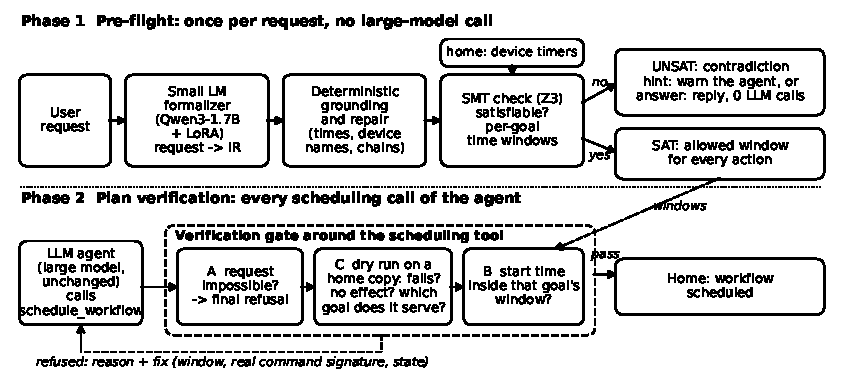
\includegraphics[width=\textwidth]{figures/architecture.pdf}
  \caption{\sys{}. Phase 1 runs once per request without any large-model call: a small LM formalizes the request,
  deterministic rules ground it, device finish times are read from the home, and Z3 either proves a contradiction
  (answered directly, or passed to the agent as a hint) or computes a time window for every goal. Phase 2 wraps
  the agent's scheduling tool: every call is checked (A) against the verdict, (C) by a dry run on a copy of the
  home, and (B) against the window of the goal it serves. Refused calls return to the agent with the fix.}
  \Description{Two-phase pipeline: pre-flight formalization and SMT check, then a gate with three checks around
  the agent's scheduling tool.}
  \label{fig:arch}
\end{figure*}

\sys{} has two phases (Figure~\ref{fig:arch}). Phase~1 decides the request once, before the agent's first step.
Phase~2 verifies every scheduling call the agent makes. The agent itself, its prompt and its tools are unchanged;
\sys{} only replaces the implementation behind the scheduling tool and, in Phase~1, may prepend a note to the
request or answer it.

\subsection{Formalizing the Request with a Small Model}\label{sec:formalize}

A small language model (Qwen3-1.7B~\cite{yang2025qwen3} with LoRA adapters~\cite{hu2022lora}) maps the request
to a compact JSON IR that lists, per goal, the target assertions and the time readings with their anchors. For
example, ``turn on kitchen fan 1 and set it to 30\% 20 minutes from now and increase it to 50\% 23 minutes after
the previous action'' becomes two goals on the fan with readings \textit{after(now, 20)} and
\textit{after(goal$_1$, 23)}. Training labels are generated automatically from each benchmark episode's ground
truth, so no manual annotation is needed. Because the IR is parsed once per request and cached, the parser adds
no latency to the agent's loop.

The parse is then passed through deterministic grounding and repair rules that encode properties of the
request, not of individual episodes. A clock time is kept only if it is stated in the text (in digits or words),
and a clock time stated with AM/PM that the parser omitted is restored. Device identifiers that do not exist in
the home are mapped to the closest existing device in the same room. A chained reading is attached to the
previous action on the \emph{same} device (``raise \emph{it} to 50\% \dots\ after the previous action''), and a
chain the parser split into two readings (``now${}+8$'' and ``previous${}+0$'') is merged. These rules are
cheap, auditable and independent of the large agent.

\subsection{Pre-flight Satisfiability Check}

Each goal $g_i$ receives a real variable $t_i$, its start time in minutes after the request. Anchors are
resolved as follows: \textit{now} is $0$; a stated clock time is its offset from the current clock; a goal anchor
is the other goal's variable $t_j$; a device anchor is the device's finish time
$\tau_d = \mathit{now} + \mathit{CountdownTime}_d/60$, which \sys{} reads from the home itself with a single tool
call and no LLM. Each reading becomes a linear constraint with tolerance $\varepsilon$:
\begin{align*}
\textit{after}(\alpha,\delta)&:\ |t_i - (A_\alpha + \delta)| \le \varepsilon, &
\textit{before}(\alpha,\delta)&:\ |t_i - (A_\alpha - \delta)| \le \varepsilon,\\
\textit{at}(\alpha)&:\ |t_i - A_\alpha| \le \varepsilon, &
\textit{by}(\alpha,\delta)&:\ t_i \le A_\alpha - \delta + \varepsilon,
\end{align*}
where $A_\alpha$ is the resolved anchor time; a clock time known only to the minute is widened by one minute.
All readings of all goals are encoded \emph{jointly}, so chained goals and goals sharing a device anchor must
agree. Z3 decides the conjunction. If it is unsatisfiable, the unsatisfiable core identifies the clashing
readings, which are turned into a plain-language explanation that states every device's actual finish time.
If it is satisfiable, Z3's optimizer computes for each goal the window $W_i=[\min t_i,\max t_i]$ of start times
consistent with the whole request.

On a contradiction, \sys{} acts in one of two modes. In \emph{hint} mode it appends the explanation to the request
and lets the agent respond (one large-model call is typically enough). In \emph{answer} mode it replies to the
user directly with the explanation and the timer readings it relied on, and the large model is never called.

\subsection{Plan Verification at the Tool Boundary}

For a feasible request, the agent proceeds as usual. Each call $\textsc{schedule}(s,\sigma)$ is intercepted and
checked in three steps; the call reaches the real home only if all pass.

\paragraph{(A) Infeasible request.} If Phase~1 proved a contradiction, the call is refused with an explanation
stating that no start time can satisfy the request and that the agent should reply to the user.

\paragraph{(C) Dry run on a copy of the home.} \sys{} takes a snapshot of the home, rebuilds it with the
simulator's own initialization code, replays the workflows already committed in the episode, schedules the
candidate and fast-forwards to its due time. A twin copy without the candidate is advanced to the same moment.
The difference between the two copies is the call's \emph{effect}. The call is refused if a step fails, with
the simulator's full reason and the cluster's real command signatures and writable attributes
(e.g., \texttt{MoveToLevel(Level, TransitionTime, ...)} when the agent wrote \texttt{\{"level": 60\}}); this
information exists in the simulator but is not visible to the agent through the benchmark's tools. The call is
also refused if it has no effect while no goal is already met, which typically means a precondition is missing
(e.g., pausing a washer that never started). Finally, the effect determines which goal the call serves: the goal
whose target values the call actually changes.

\paragraph{(B) Time check.} A call matched to goal $g_i$ is refused if it starts after $W_i$ ends, or if it would
overwrite an earlier goal on the same device before that goal is checked. For an ordinary earlier goal this bound
is the start of its window; for a \emph{deadline} goal (relation \textit{by}, e.g., ``still running one minute
before the dryer finishes'') it is the deadline itself, because the goal is checked at that instant. A call
whose effect matches no goal is not time-checked, so a goal missed by the parser cannot cause a refusal.
Refusals state the allowed range and the device finish times it derives from.

\paragraph{Bounded interference.} Each refusal type is issued at most $k=2$ times per episode; afterwards calls
pass, annotated with the remaining concern. The gate therefore adds at most a constant number of agent turns and
can never trap the agent in a loop, and any failure inside the gate fails open.

\subsection{Properties}

\textit{Soundness of contradiction verdicts.} If the IR faithfully represents the request and the device timers
are read correctly, an UNSAT verdict implies that no schedule satisfies the request; the verdict is a proof,
not a judgment by the agent. Errors therefore come only from formalization, which we measure separately.
\textit{Black-box applicability.} \sys{} needs only the agent's tool interface; it works with hosted models whose
decoding cannot be controlled. \textit{Cost.} Phase~1 needs no large-model call; solving takes about 0.1\,s per
request and all dry runs of an episode a few seconds.

%%%%%%%%%%%%%%%%%%%%%%%%%%%%%%%%%%%%%%%%%%%%%%%%%%%%%%%%%%%%%%%%%%%%%%%%%%%%%%%%%%%%%%%%%%%%%%%%%%%%%%%%%%%%%%%%
\section{Experimental Setup}

\paragraph{Benchmark and agent.} We use all 300 QT4 episodes of SimuHome. Fourteen QT4-3 infeasible episodes are
conflicts between a device's run-time model and a pause request; they are outside \sys{}'s temporal formalization
and are reported but counted as out of scope. The agent is SimuHome's ReAct agent with its default step limit,
at temperature 0. The main evaluation uses Qwen2.5-14B-Instruct (4-bit, served locally with Ollama on two T4
GPUs), a non-reasoning instruction-tuned model; the preliminary runs used Gemma-4-31B-it through a hosted API,
which became unavailable during the study. Feasible episodes are scored by SimuHome's simulator alone: the
home's state is checked at each goal's time, so no LLM judgment is involved. Infeasible episodes are scored by
SimuHome's panel of three LLM judges, here three votes of the agent's own model; SimuHome reads only the first
letter of each verdict, which rules out reasoning models as judges. All arms share the same judge.

\paragraph{Arms.} We compare four configurations on the same episodes: the agent alone; the agent with a one-line
\emph{self-check} instruction to verify all times and report contradictions; \sys{} in hint mode; and \sys{} in
answer mode (impossible requests only, since on possible requests it differs from hint mode only when the parser
wrongly reports a contradiction).

\paragraph{Parser.} The parser is trained with 5-fold cross-validation over episode seeds, so every request is
parsed by a model that never saw it during training (LoRA rank 16, 5 epochs, best epoch by validation loss).

\paragraph{Latency control.} SimuHome's home runs in real time, the agent is told the current time once, and
the scorer evaluates goals only from the tick at which the episode ends. With a hosted API taking 65--80\,s per
call, episodes lasted 6--13 minutes: start times expired before submission, and plans built on the stale clock
were minutes early, independently of the method. We therefore stop each simulator's clock while its agent waits
for an LLM response, for all arms alike. Tool calls, the gate's own work and the scorer run on the normal clock.

\paragraph{Metrics.} Success rate per (sub-type, case), goals met on feasible requests, and large-model calls
per episode. Arms are compared episode by episode with McNemar's exact test~\cite{mcnemar1947}. SimuHome marks an
episode as an infrastructure error, not a failure, when the agent exhausts its steps without a final answer or
a service fails; we count these as failures (strict scoring). Excluding them instead gives the same conclusions.

%%%%%%%%%%%%%%%%%%%%%%%%%%%%%%%%%%%%%%%%%%%%%%%%%%%%%%%%%%%%%%%%%%%%%%%%%%%%%%%%%%%%%%%%%%%%%%%%%%%%%%%%%%%%%%%%
\section{Results}

\subsection{Formalization Quality}

Table~\ref{tab:parser} scores the 5-fold parses as the gate uses them. Every scored possible request is judged
possible, so the pre-flight check never tells the agent that a feasible request is impossible. Contradictions in
QT4-1 and QT4-2 are almost all proven; in QT4-3, 30 of 36 in-scope contradictions are proven, the remainder
using phrasings the grounding rules do not cover. A correct schedule would be refused by the time check for one
of 247 benchmark goals (a parse that merged two steps). Only 56\% of the IRs match the reference exactly, yet the
verdicts are almost always right: most differences (e.g., goal order, an extra redundant reading) do not change
the constraint system.

\begin{table}[t]
  \caption{Formalization quality with 5-fold cross-validated parses (gate preprocessing applied). Two of 300
  parses were not valid JSON; the gate lets those episodes through unchecked.}
  \label{tab:parser}
  \centering\small
  \begin{tabular}{lccc}
    \toprule
     & QT4-1 & QT4-2 & QT4-3 \\
    \midrule
    Possible judged possible & 49/49 & 49/49 & 50/50 \\
    Contradictions proven (in scope) & 49/50 & 50/50 & 30/36 \\
    Correct schedules refused (goals) & 1/148 & 0/49 & 0/50 \\
    \bottomrule
  \end{tabular}
\end{table}

\subsection{Main Result: Full Paired Evaluation}\label{sec:main}

Table~\ref{tab:full} reports the latency-controlled evaluation on all 300 episodes (about 50 per cell) with the
Qwen2.5-14B agent; every arm ran on the same episodes.

\begin{table}[t]
  \caption{Full paired evaluation (Qwen2.5-14B agent, strict scoring). Large-model calls per episode in
  parentheses. *14 of 50 impossible QT4-3 episodes are out of scope (maximum 36/50).}
  \label{tab:full}
  \centering\small
  \setlength{\tabcolsep}{4pt}
  \begin{tabular}{llccc}
    \toprule
    Case & Arm & QT4-1 & QT4-2 & QT4-3 \
    \midrule
    \multirow{3}{*}{Possible} & Agent alone & 0/49 & 2/49 & 0/50 \
     & Self-check & 0/49 & 1/49 & 0/50 \
     & \sys{} & \textbf{6/49} & \textbf{9/49} & 0/50 \
    \midrule
    \multirow{4}{*}{Impossible} & Agent alone & 3/50 (4.3) & 5/50 (7.1) & 1/50* (7.5) \
     & Self-check & 5/50 (4.3) & 11/50 (7.6) & 3/50* (7.7) \
     & \sys{}, hint & \textbf{49/50} (1.1) & \textbf{50/50} (2.0) & \textbf{30/50}* (4.9) \
     & \sys{}, answer & \textbf{49/50} (0.1) & \textbf{50/50} (0.0) & \textbf{31/50}* (3.1) \
    \bottomrule
  \end{tabular}
\end{table}

\paragraph{Impossible requests.} \sys{} handles 129 (hint) and 130 (answer) of 150 contradictory requests
correctly, against 9 for the agent alone and 19 with the self-check prompt ($p<10^{-30}$ for each comparison,
McNemar, pooled; $p<10^{-7}$ in every sub-type). In answer mode, QT4-1 and QT4-2 need 0.1 and 0 large-model
calls per request; on QT4-3 the agent is still called when the parser does not prove the contradiction. With
this agent, unlike with the larger Gemma-4-31B (Table~\ref{tab:prelim}), the self-check prompt no longer helps:
prompting depends on the agent's own temporal reasoning, while \sys{}'s verdict does not. The judge is
not error-free in either direction that matters here: in 18 impossible-request episodes it accepted an answer
although the agent had scheduled actions anyway, 17 of them for the agent alone or with self-check. Counting
these as failures lowers the baselines to 2 and 9 of 150 and leaves \sys{} at 129, so the reported gap is
conservative. The pre-flight check
called none of the 131 logged possible requests impossible.

\paragraph{Possible requests.} The agent alone completes 2 of 148 feasible requests and 1 with self-check;
\sys{} completes 15 ($p<0.001$ against both, pooled; QT4-1: $p=0.03$, QT4-2: $p=0.02$--$0.04$). The gain is larger in partial progress: on QT4-1, 56 of 138 benchmark goals are met
with \sys{} against 19 of 148 for the agent alone and 15 of 142 with self-check. In 13 of the 14 episodes that
only \sys{} completed, the gate had refused a failing step and returned the device's real command signature or
writable attributes (e.g., \texttt{MoveToLevel(Level, \dots)}, a read-only \texttt{TemperatureSetpoint}, or
\texttt{DownOrClose} for a window covering that has no \texttt{Close} command); two also involved a time
refusal and two a no-effect refusal. No arm completes a feasible QT4-3 request, which requires coordinating two
devices' run times; this agent does not manage it with or without feedback.

\paragraph{Cost and errors.} Gate checks add about one to four agent turns per feasible episode (refusals the
agent answers). Infrastructure errors (mostly the agent running out of steps) affect 12 runs for the agent
alone, 25 with self-check, 14 for \sys{} in hint mode and 3 in answer mode, out of 300 or 150 per arm.

\subsection{A Larger Agent: Preliminary Contradiction Detection}

To see how the picture changes with a stronger agent, Table~\ref{tab:prelim} reports an earlier run with
Gemma-4-31B on the held-out split of the first fold (54 episodes), made with an earlier version of the gate
(without the repairs of Section~\ref{sec:formalize}) and before latency control. Alone, the
agent detects 4 of 10 QT4-1 and none of 8 QT4-2 contradictions, consistent with the contradiction blindness
reported for SimuHome. \sys{} detects all of them; in answer mode with zero large-model calls, and in hint mode
with one to two. Episode by episode, answer mode is significantly better than the agent alone
($p=0.002$, McNemar, all three sub-types pooled). A self-check prompt reaches the same accuracy with this agent,
but at 1.1 to 3.5 large-model calls per request, and without a proof; with the 14B agent of
Section~\ref{sec:main} the same prompt fails, while \sys{}'s verdicts are unchanged. On QT4-3, 5 of the 9 contradictions in this
split are run-time conflicts outside the formalization, so 4 of 9 is the attainable maximum.

\begin{table}[t]
  \caption{Preliminary: impossible requests correctly handled (54 held-out episodes) and large-model calls per
  request. *5 of 9 QT4-3 cases are out of scope (maximum 4/9).}
  \label{tab:prelim}
  \centering\small
  \begin{tabular}{lcccc}
    \toprule
    Arm & QT4-1 & QT4-2 & QT4-3* & Calls (QT4-1/2) \\
    \midrule
    Agent alone & 4/10 & 0/8 & 4/9 & 3.1 / 6.9 \\
    Self-check prompt & 10/10 & 8/8 & 5/9 & 1.1 / 3.5 \\
    \sys{}, hint & 10/10 & 8/8 & 4/9 & 1.0 / 2.0 \\
    \sys{}, answer & 10/10 & 8/8 & 4/9 & 0 / 0 \\
    \bottomrule
  \end{tabular}
\end{table}

\subsection{Plan Verification on Real Agent Traces}

To measure the gate's decisions independently of the agent's subsequent behaviour, we replayed all 188 scheduling
calls that the agent made in 91 possible-request episodes of the preliminary runs through the current gate, with
the cross-validated parses, in-process copies of each home and the agent's own action order. The gate flags the
agent's mistake in 52 of 62 failed episodes. It would block a call in one of 29 successful episodes; there, the
time window comes from a garbled parse, and the bounded-interference rule would let the call through after at
most two refusals.

\subsection{Why Agents Fail on Feasible Requests}

Re-simulating every failed feasible run of the preliminary experiments (all arms) from the agent's own actions
shows that timing is rarely the problem in QT4-1 and QT4-2. In 36 of 40 failed runs the agent issued at least one device command that could
not produce the requested state: wrong argument names (16 runs, e.g., \texttt{level} for \texttt{Level}),
writes to read-only attributes (8), wrong value scales (6), non-existent commands or attributes (6), wrong mode
values (5) and thermostat deadband violations (4). The scheduling tool accepts all of these, so the agent never
learns about them. In QT4-3 the agent computed the coordinating device's finish time from a stale clock, pausing
1--5 minutes early in all 8 scheduled cases. Both error types are exactly what checks (C) and (B) target.

%%%%%%%%%%%%%%%%%%%%%%%%%%%%%%%%%%%%%%%%%%%%%%%%%%%%%%%%%%%%%%%%%%%%%%%%%%%%%%%%%%%%%%%%%%%%%%%%%%%%%%%%%%%%%%%%
\section{Conclusion and Limitations}

We presented \sys{}, a verification layer in which a small language model and an SMT solver check both the
request and the plan of an unmodified LLM agent before anything is executed in the home. Contradictory requests
are decided by proof and can be answered without any large-model call; scheduling calls are checked against
request-derived time windows and a dry run of the home, and refused with fixes the agent can act on. The method
addresses the failure modes identified for current smart-home agents, contradiction blindness and the absence
of feedback after scheduling, while leaving the agent and its tools untouched. On 300 paired episodes it
turns a 14B agent that handles 6\% of contradictory requests into a system that handles 87\%, mostly without
calling the large model, and it is the only configuration that completes feasible requests at a non-trivial
rate, by telling the agent exactly how to fix the commands it gets wrong.

\paragraph{Limitations.} (i) \emph{One benchmark and one language style.} All results are on SimuHome, whose
requests are generated from templates, and the parser is trained on the same style; robustness to free-form
phrasing is untested. (ii) \emph{Rules informed by the benchmark.} The grounding rules were designed after
inspecting parse errors on these episodes. Each encodes a general property of requests and agrees with the
benchmark's labels, but they should be validated on unseen phrasings. (iii) \emph{Scope of the formalization.}
Conflicts that depend on device run-time models (14 QT4-3 episodes) and phrasings outside the grounding rules
are not detected. (iv) \emph{Simulation.} The dry run requires a simulator or digital twin of the home; in a
physical home it is only as accurate as that model. (v) \emph{Evaluation protocol.} We pause the simulator's
clock during LLM calls to remove hosted-API latency, a deviation from SimuHome's real-time protocol applied to
all arms alike. (vi) \emph{Agents.} With the larger Gemma-4-31B agent a self-check prompt matched \sys{} on
impossible requests (preliminary run); the full evaluation uses a single 14B agent, whose absolute success on
feasible requests remains low even with \sys{}, and none of the arms solves feasible QT4-3. Evaluating larger
agents on the full protocol, free-form requests and other device domains is future work. (vii) \emph{Judge.}
Impossible requests are scored by the agent's own model; all arms share this judge, and feasible requests involve
no judge at all, but re-scoring with an independent judge and a manual audit of a sample of verdicts remain to be
done.

\begin{acks}
Omitted for anonymous review.
\end{acks}

\balance
\bibliographystyle{ACM-Reference-Format}
\bibliography{references}

\end{document}
